\documentclass{jsarticle}
\usepackage[dvipdfmx]{graphicx}
\usepackage{here}
\begin{titlepage}
\title{Arduino Pulse Generator Readme}
\author{Yuzuki Mimura}
\date{}
\begin{document}
\maketitle
\end{titlepage}

\section{Setup}
This device can be set threthord and pulse length.\\
In order to set up this, you can use 2 jumper pin like select button and Ener button.\\
As shown in the figure below, use jumper pin "N" to select value, "R" to Enter.\\
\begin{figure}[H]
\begin{center} 
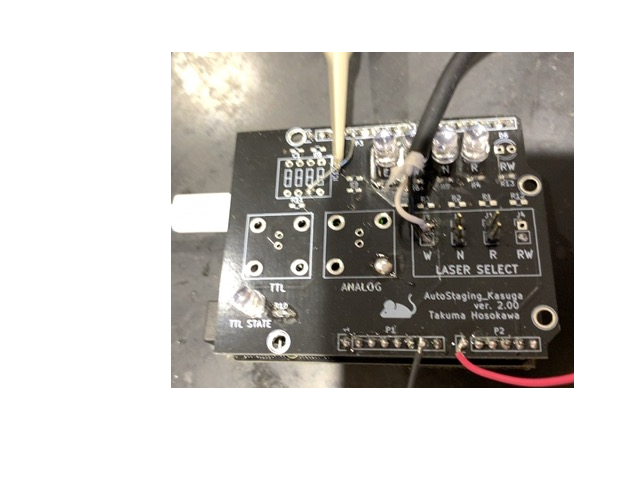
\includegraphics[scale = 0.6]{pic1.png}
\caption{Jumper Pin}
\end{center}
\end{figure}

When you turn on the power, setup mode will start. If you don't want to setup , you dont have to do anything. \\
\\
Setup mode have 2 stage of setup. first,you can set threthord. Short jumper "N" sometime to select threthord,and short jumper "R"  once and short timeto decide value.\\
After this , you can set pulse length in the same way. When setting is completed, LED "E" will blink. The setting is over with this.\\
\begin{figure}[H]
\begin{center} 
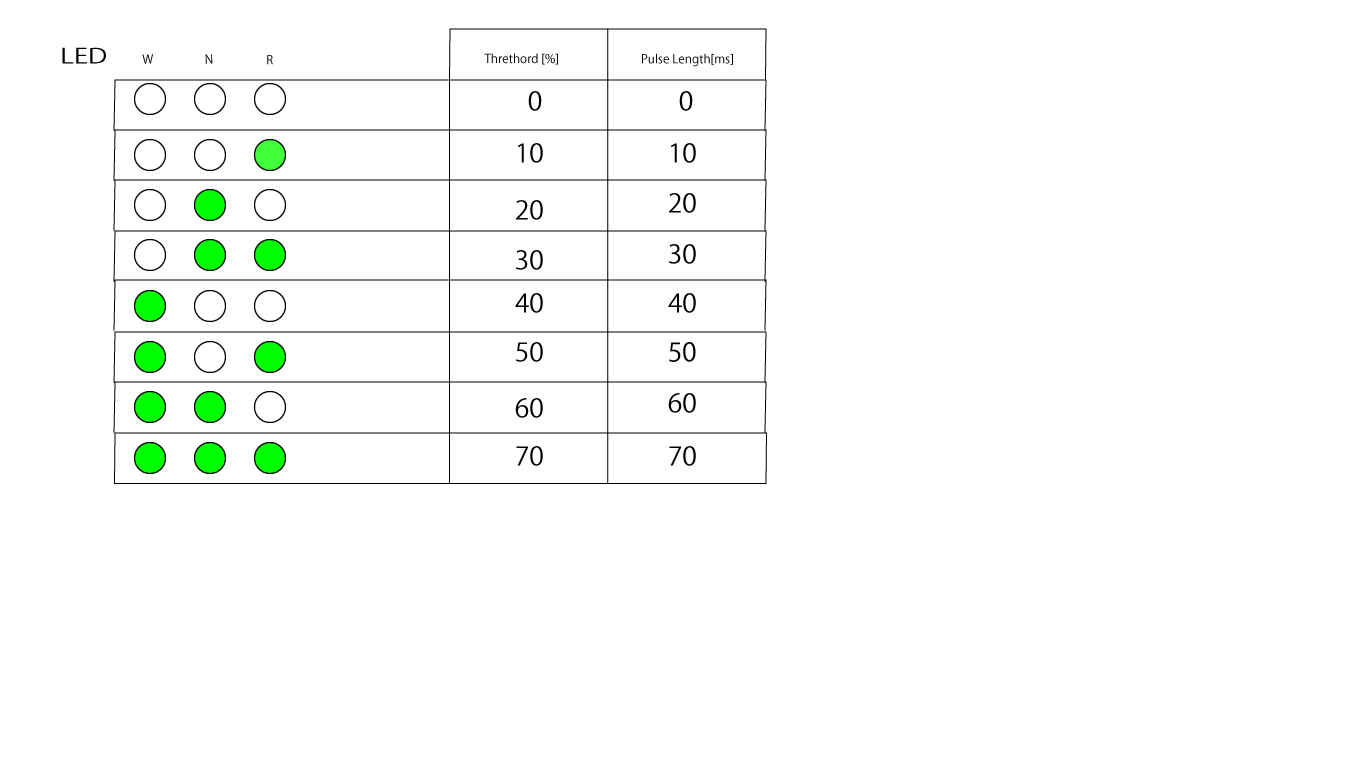
\includegraphics[scale = 0.6]{led.png}
\caption{LED binary table}
\end{center}
\end{figure}
\newpage

\section{RUN}
work in progress
\end{document}
    


